\documentclass[14pt,a4paper,report]{report}
\usepackage[a4paper, mag=1000, left=2.5cm, right=1cm, top=2cm, bottom=2cm, headsep=0.7cm, footskip=1cm]{geometry}
\usepackage[utf8]{inputenc}
\usepackage[english,russian]{babel}
\usepackage{indentfirst}
\usepackage[dvipsnames]{xcolor}
\usepackage[colorlinks]{hyperref}
\usepackage{listings} 
\usepackage{fancyhdr}
\usepackage{caption}
\usepackage{amsmath}
\usepackage{latexsym}
\usepackage{graphicx}
\usepackage{amsmath}
\hypersetup{
	colorlinks = true,
	linkcolor  = black
}

\usepackage{titlesec}
\titleformat{\chapter}
{\Large\bfseries} % format
{}                % label
{0pt}             % sep
{\huge}           % before-code


\DeclareCaptionFont{white}{\color{white}} 

% Listing description
\usepackage{listings} 
\DeclareCaptionFormat{listing}{\colorbox{gray}{\parbox{\textwidth}{#1#2#3}}}
\captionsetup[lstlisting]{format=listing,labelfont=white,textfont=white}
\lstset{ 
	% Listing settings
	inputencoding = utf8,			
	extendedchars = \true, 
	keepspaces = true, 			  	 % Поддержка кириллицы и пробелов в комментариях
	language = Matlab,            	 	 % Язык программирования (для подсветки)
	basicstyle = \small\sffamily, 	 % Размер и начертание шрифта для подсветки кода
	numbers = left,               	 % Где поставить нумерацию строк (слева\справа)
	numberstyle = \tiny,          	 % Размер шрифта для номеров строк
	stepnumber = 1,               	 % Размер шага между двумя номерами строк
	numbersep = 5pt,              	 % Как далеко отстоят номера строк от подсвечиваемого кода
	backgroundcolor = \color{white}, % Цвет фона подсветки - используем \usepackage{color}
	showspaces = false,           	 % Показывать или нет пробелы специальными отступами
	showstringspaces = false,    	 % Показывать или нет пробелы в строках
	showtabs = false,           	 % Показывать или нет табуляцию в строках
	frame = single,              	 % Рисовать рамку вокруг кода
	tabsize = 2,                  	 % Размер табуляции по умолчанию равен 2 пробелам
	captionpos = t,             	 % Позиция заголовка вверху [t] или внизу [b] 
	breaklines = true,           	 % Автоматически переносить строки (да\нет)
	breakatwhitespace = false,   	 % Переносить строки только если есть пробел
	escapeinside = {\%*}{*)}      	 % Если нужно добавить комментарии в коде
}

\begin{document}

\def\contentsname{Содержание}

% Titlepage
\begin{titlepage}
	\begin{center}
		\textsc{Санкт-Петербургский Политехнический 
			Университет Петра Великого\\[5mm]
			Кафедра компьютерных систем и программных технологий}
		
		\vfill
		
		\textbf{Отчёт по лабораторной работе №2\\[3mm]
			Курс: «Теория автоматического управления»\\[3mm]
			Тема: «Изучение различных форм представления системы»\\[35mm]
			}
	\end{center}
	
	\hfill
	\begin{minipage}{.5\textwidth}
		Выполнил студент:\\[2mm] 
		Раскин Андрей Романович	\\
		Группа: 43501/3\\[5mm]
		
		Проверил:\\[2mm] 
		Нестеров Сергей Александрович
	\end{minipage}
	\vfill
	\begin{center}
		Санкт-Петербург\\ \the\year\ г.
	\end{center}
\end{titlepage}

% Contents
\tableofcontents
\clearpage

\chapter{Лабораторная работа №2}

\section{Цель работы}

Получить навыки работы с моделями ВСВ и каноническими представлениями.

\section{Программа работы}

\begin{itemize}
	\item Представить систему в трех канонических формах.
	\item Получить структурные схемы для каждой формы.
	\item Получить матрицы управляемости и матрицы преобразования.
	\item Проверить систему на устойчивость, наблюдаемость и управляемость.
\end{itemize}

\section{Индивидуальное задание}

$a_0=0.75,a_1=2,b_0=0,b_1=1,  y(0)=0, y'(0)=0, u=1(t)$
\\
$
x''+2x'+0.75x=u'
$


\section{Ход работы}

\subsection{Построение канонических форм}

\subsubsection{Нормальная форма управления}

\begin{equation*}
\text{$W(p)=\frac{p}{p^2+2p+0.75}=\frac{y}{u}$}
\end{equation*}

\begin{equation*}
\text{$\frac{y}{p}=\frac{u}{p^2+2p+0.75}=x_1$}
\Longrightarrow
\begin{cases}
	\text{$u=x_1(p^2+2p+0.75)$} \\
	\text{$y=x_1(p)$}
\end{cases}
\end{equation*}

\begin{equation*}
\begin{cases}
	\text{$px_1=x_2$} \\
	\text{$px_2=u-2p*x_2-0.75x_1$}\\
	\text{$y=x_2$}
\end{cases}
\end{equation*}

\begin{equation*}
\text{$A=$}
\text{$
\begin{bmatrix}
0 & 1 \\
-0.75 & -2 \\
\end{bmatrix}
$}
\text{$, B=$}
\text{$
\begin{bmatrix}
0 \\
1 \\
\end{bmatrix}
$}
\text{$, C=$}
\text{$
\begin{bmatrix}
0 & 1 \\
\end{bmatrix}
$}
\end{equation*}

Проверим корректность полученных матриц $A, B, C$:

\begin{equation*}
\text{$det(A-\lambda)=0$}
\Longrightarrow
\text{$-\lambda(-2-\lambda) + 0.75=0$}
\Longrightarrow
\begin{cases}
	\text{$\lambda_1=-3/2$} \\
	\text{$\lambda_2=-1/2$}
\end{cases}
\end{equation*}

Собственные числа совпадают с собственными числами матриц в нормальной форме наблюдения и канонической форме, что свидетельствует о корректности полученных матриц  $A, B, C$.

\begin{equation*}
\text{$W(p)=C(pE-A)^{-1}B=
\begin{bmatrix}
0 & 1 \\
\end{bmatrix}
\begin{bmatrix}
p & -1 \\
0.75 & p+2\\
\end{bmatrix}^{-1}
\begin{bmatrix}
0 \\
1 \\
\end{bmatrix}=
\begin{bmatrix}
0 & 1 \\
\end{bmatrix}
\begin{bmatrix}
\frac{4*(p + 2)}{4*p^2 + 8*p + 3} & \frac{4}{4*p^2 + 8*p + 3} \\
\frac{-3}{4*p^2 + 8*p + 3}& \frac{4p}{4*p^2 + 8*p + 3}\\
\end{bmatrix}
\begin{bmatrix}
0 \\
1 \\
\end{bmatrix}=
$}
\end{equation*}

\begin{equation*}
\text{$=\begin{bmatrix}
	\frac{-3}{4*p^2 + 8*p + 3} & \frac{4p}{4*p^2 + 8*p + 3} \\
	\end{bmatrix}\begin{bmatrix}
	0 \\
	1 \\
	\end{bmatrix}=\frac{p}{p^2+2p+0.75}
	$}
\end{equation*}

Передаточная функция, полученная в результате преобразования $W(p)=C(pE-A)^{-1}B$, полностью совпадает с исходной, что свидетельствует о корректности полученных матриц  $A, B, C$. 


\begin{figure}[h!]
	\centering
	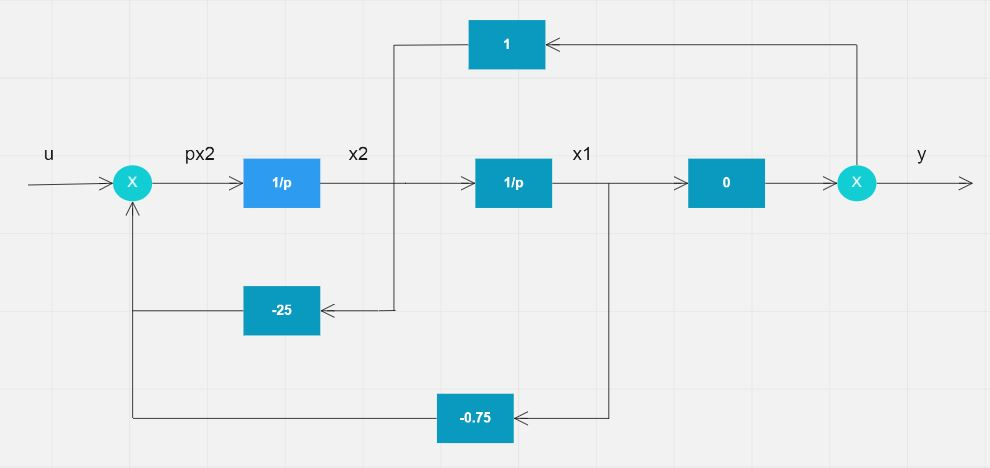
\includegraphics[scale = 0.6]{images/nfu.jpg}
	\caption{Структурная схема НФУ}
	\label{image:1}
\end{figure}

\subsubsection{Нормальная форма наблюдения}

\begin{equation*}
\text{$W(p)=\frac{p}{p^2+2p+0.75}=\frac{y}{u}$}
\Longrightarrow
\text{$pu=(p^2+2p+0.75)y$}
\Longrightarrow
\end{equation*}

\begin{equation*}
\Longrightarrow
\text{$p^2y+2py+0.75y - pu =0$}
\Longrightarrow
\text{$p(p(y)+2y-u)++0.75y=0$}
\end{equation*}

\begin{equation*}
\begin{cases}
	\text{$x_1=py+2y-u$} \\
	\text{$px_1=-0.75y$} \\
\end{cases}
\Longrightarrow
\begin{cases}
	\text{$x_2=y$}\\
	\text{$x_1=px_2+2x_2-u$} \\
	\text{$px_1=0.75x_2$} \\
\end{cases}
\Longrightarrow
\begin{cases}
	\text{$px_1=0.75x_2$} \\
	\text{$px_2=x_1-2x_2+u$} \\
	\text{$y=x_2$}
\end{cases}
\end{equation*}

\begin{equation*}
\text{$A=$}
\text{$
	\begin{bmatrix}
	0 & -0.75 \\
	1 & -2 \\
	\end{bmatrix}
	$}
\text{$, B=$}
\text{$
	\begin{bmatrix}
	0 \\
	1 \\
	\end{bmatrix}
	$}
\text{$, C=$}
\text{$
	\begin{bmatrix}
	0 & 1 \\
	\end{bmatrix}
	$}
\end{equation*}

Проверим корректность полученных матриц $A, B, C$:

\begin{equation*}
\text{$det(A-\lambda)=0$}
\Longrightarrow
\text{$-\lambda(-2-\lambda) + 3/4=0$}
\Longrightarrow
\begin{cases}
	\text{$\lambda_1=-1/2$} \\
	\text{$\lambda_2=-3/2$}
\end{cases}
\end{equation*}

Собственные числа совпадают с собственными числами матриц в нормальной форме управления и канонической форме, что свидетельствует о корректности полученных матриц  $A, B, C$.

\begin{equation*}
\text{$W(p)=C(pE-A)^{-1}B=
\begin{bmatrix}
0 & 1 \\
\end{bmatrix}
\begin{bmatrix}
p & 3/4 \\
-1 & p+2\\
\end{bmatrix}^{-1}
\begin{bmatrix}
0 \\
1 \\
\end{bmatrix}=
\begin{bmatrix}
0 & 1 \\
\end{bmatrix}
\begin{bmatrix}
\frac{4*(p + 2)}{4*p^2 + 8*p + 3} & \frac{-3}{4*p^2 + 8*p + 3} \\
\frac{4}{4*p^2 + 8*p + 3} & \frac{4p}{4*p^2 + 8*p + 3}\\
\end{bmatrix}
\begin{bmatrix}
0 \\
1 \\
\end{bmatrix}=
$}
\end{equation*}

\begin{equation*}
\text{$=\begin{bmatrix}
\frac{4}{4*p^2 + 8*p + 3} & \frac{4p}{4*p^2 + 8*p + 3} \\
\end{bmatrix}\begin{bmatrix}
0 \\
1 \\
\end{bmatrix}=\frac{p}{p^2+2p+0.75}
$}
\end{equation*}

Передаточная функция, полученная в результате преобразования $W(p)=C(pE-A)^{-1}B$, полностью совпадает с исходной, что свидетельствует о корректности полученных матриц  $A, B, C$. 

\clearpage

\begin{figure}[h!]
	\centering
	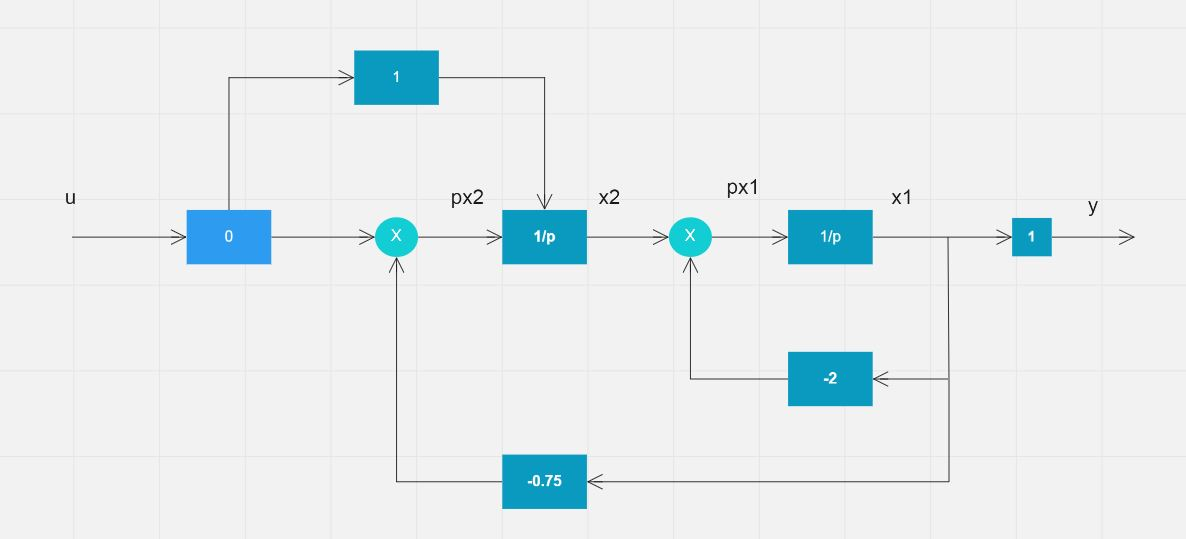
\includegraphics[scale = 0.5]{images/nfn.jpg}
	\caption{Структурная схема НФН}
	\label{image:2}
\end{figure}

\subsubsection{Каноническая форма}

\begin{equation*}
\text{$W(p)=\frac{p}{p^2+2p+0.75}=\frac{p}{(p+1/2)(p+3/2)}=\frac{1.5}{p+3/2}-\frac{0.5}{p+1/2}=\frac{y}{u}$}
\end{equation*}

\begin{equation*}
\begin{cases}
	\text{$\frac{x_1}{u}=\frac{1.5}{p+3/2}$} \\
	\text{$\frac{x_2}{u}=\frac{-0.5}{p+1/2}$} \\
	\text{$y=x_1+x_2$}
\end{cases}
\Longrightarrow
\begin{cases}
\text{$px_1=1.5-3/2x_1$} \\
\text{$px_2=-1/2x_2-1/2u$} \\
\text{$y=x_1+x_2$}
\end{cases}
\end{equation*}

\begin{equation*}
\text{$A=$}
\text{$
	\begin{bmatrix}
	-3/2 & 0 \\
	0 & -1/2 \\
	\end{bmatrix}
	$}
\text{$, B=$}
\text{$
	\begin{bmatrix}
	1.5 \\
	-0.5 \\
	\end{bmatrix}
	$}
\text{$, C=$}
\text{$
	\begin{bmatrix}
	1 & 1 \\
	\end{bmatrix}
	$}
\end{equation*}

Проверим корректность полученных матриц $A, B, C$:

\begin{equation*}
\text{$det(A-\lambda)=0$}
\Longrightarrow
	\text{$(-3/2-\lambda)(-1/2-\lambda) + \lambda^2=0$}
\Longrightarrow
\begin{cases}
	\text{$\lambda_1=-1/2$} \\
	\text{$\lambda_2=-3/2$}
\end{cases}
\end{equation*}

Собственные числа совпадают с собственными числами матриц в нормальной форме управления и нормальной форме наблюдения, что свидетельствует о корректности полученных матриц  $A, B, C$

\begin{equation*}
\text{$W(p)=C(pE-A)^{-1}B=
	\begin{bmatrix}
	1 & 1 \\
	\end{bmatrix}
	\begin{bmatrix}
	p+3/2 & 0 \\
	0 & p+1/2\\
	\end{bmatrix}^{-1}
	\begin{bmatrix}
	1.5 \\
	-0.5 \\
	\end{bmatrix}=
	\begin{bmatrix}
	1 & 1 \\
	\end{bmatrix}
	\begin{bmatrix}
	\frac{4*(p + 2)}{4*p^2 + 8*p + 3} & \frac{-3}{4*p^2 + 8*p + 3} \\
	\frac{4}{4*p^2 + 8*p + 3} & \frac{4p}{4*p^2 + 8*p + 3}\\
	\end{bmatrix}
	\begin{bmatrix}
	1.5 \\
	-0.5 \\
	\end{bmatrix}=
	$}
\end{equation*}

\begin{equation*}
\text{$=\begin{bmatrix}
	\frac{2}{2*p + 3} & \frac{2}{2*p + 1} \\
	\end{bmatrix}\begin{bmatrix}
	1,5 \\
	-0,5 \\
	\end{bmatrix}=\frac{p}{p^2+2p+0.75}
	$}
\end{equation*}

Передаточная функция, полученная в результате преобразования $W(p)=C(pE-A)^{-1}B$, полностью совпадает с исходной, что свидетельствует о корректности полученных матриц  $A, B, C$. 


\begin{figure}[h!]
	\centering
	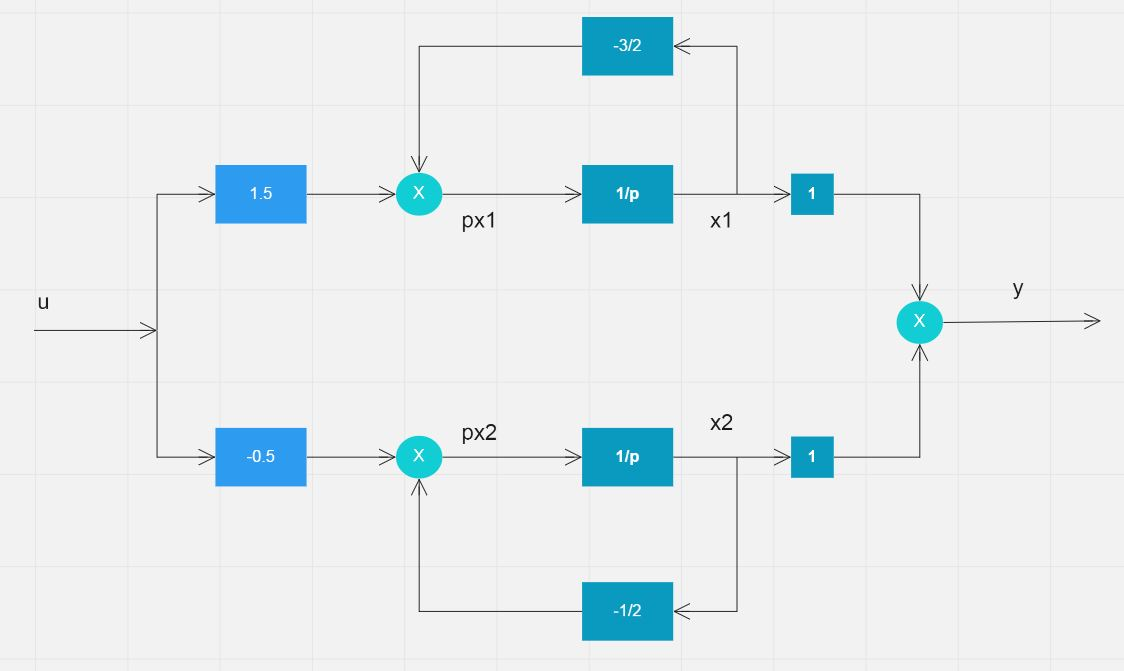
\includegraphics[scale = 0.6]{images/kf.jpg}
	\caption{Структурная схема КФ}
	\label{image:3}
\end{figure}

\subsection{Преобразования форм}

\subsubsection{Матрицы управляемости}

Матрица управляемости находится как блочная матрица, где первый столбец равен матрице $B$, а второй столбец равен произведению $AB$:

\begin{center}
$U=[B, AB]$
\end{center}

Матрицы управляемости нормальной формы управления (НФУ):

\begin{equation*}
\text{$U=\begin{bmatrix} 0 & 1 \\ 1 & -2 \end{bmatrix}$}
\text{$, U^{-1}=\begin{bmatrix} 2 & 1 \\ 1 & 0 \end{bmatrix}$}
\end{equation*}

Матрицы управляемости нормальной формы наблюдения (НФН):

\begin{equation*}
\text{$U=\begin{bmatrix} 0 & -0.75 \\ 1 & -2 \end{bmatrix}$}
\text{$, U^{-1}=\begin{bmatrix} -8/3 & 1\\ -4/3 & 0 \end{bmatrix}$}
\end{equation*}

Матрицы управляемости канонической формы (КФ):

\begin{equation*}
\text{$U=\begin{bmatrix} 1.5 & -2.25 \\ -0.5 & 0.25 \end{bmatrix}$}
\text{$, U^{-1}=\begin{bmatrix} -1/3 & -3 \\ -2/3 & -2 \end{bmatrix}$}
\end{equation*}

\subsubsection{Матрицы преобразования}

Матрица преобразования высчитывается по формуле:

\begin{center}
$P=U_{*}U^{-1}$
\end{center}

\begin{itemize}
	\item Матрица преобразования из НФУ в НФН:
	
	\begin{equation*}
	\text{$P=U_{*}U^{-1}=\begin{bmatrix} 0 & -0.75 \\ 1 & -2 \end{bmatrix}\begin{bmatrix} 2 & 1 \\ 1 & 0 \end{bmatrix}=\begin{bmatrix} -0.75 & 0 \\ 0 & 1 \end{bmatrix}$}
	\end{equation*}
	
	Проверим корректность полученной матрицы преобразования $P$. Для этого получим матрицу $B_{*}$ через матрицу $B$. 
	
	\begin{equation*}
	\text{$B_{*}=PB$}
	\Longrightarrow
	\text{$B_{*}=\begin{bmatrix} -0.75 & 0 \\ 0 & 1 \end{bmatrix}\begin{bmatrix} 0 \\ 1 \end{bmatrix}==\begin{bmatrix} 0 \\ 1 \end{bmatrix}$}
	\end{equation*}
	
	\item Матрица преобразования из НФУ в КФ:
	
	\begin{equation*}
	\text{$P=U_{*}U^{-1}=\begin{bmatrix} 1.5 & -2.5 \\ -0.5 & 0.25 \end{bmatrix}\begin{bmatrix} 2 & 1 \\ 1 & 0 \end{bmatrix}=\begin{bmatrix} 0.75 & 1.5 \\ -0.75 & -0.5 \end{bmatrix}$}
	\end{equation*}
	
	Проверим корректность полученной матрицы преобразования $P$. Для этого получим матрицу $B_{*}$ через матрицу $B$. 
	
	\begin{equation*}
	\text{$B_{*}=PB$}
	\Longrightarrow
	\text{$B_{*}=\begin{bmatrix} 0.75 & 1.5 \\ -0.75 & -0.5 \end{bmatrix}\begin{bmatrix} 0 \\ 1 \end{bmatrix}=\begin{bmatrix} 1.5 \\ -0.5 \end{bmatrix}$}
	\end{equation*}
	
	
	
	
	\item Матрица преобразования из НФН в НФУ:
	
	\begin{equation*}
	\text{$P=U_{*}U^{-1}=\begin{bmatrix} 0 & 1 \\ 1 & -2 \end{bmatrix}\begin{bmatrix} -8/3 & 1\\ -4/3 & 0 \end{bmatrix}=\begin{bmatrix} -4/3 & 0 \\ 0 & 1 \end{bmatrix}$}
	\end{equation*}
	
	Проверим корректность полученной матрицы преобразования $P$. Для этого получим матрицу $B_{*}$ через матрицу $B$.
	
	\begin{equation*}
	\text{$B_{*}=PB$}
	\Longrightarrow
	\text{$B_{*}=\begin{bmatrix} -4/3 & 0 \\ 0 & 1 \end{bmatrix}\begin{bmatrix} 0 \\ 1 \end{bmatrix}=\begin{bmatrix} 1.5 \\ -0.5 \end{bmatrix}$}
	\end{equation*}
	
	\item Матрица преобразования из НФН в КФ:
	
	\begin{equation*}
	\text{$P=U_{*}U^{-1}=\begin{bmatrix} 1.5 & -2.25 \\ -0.5 & 0.25 \end{bmatrix}\begin{bmatrix} -8/3 & 1\\ -4/3 & 0 \end{bmatrix}=\begin{bmatrix} -1 & 1.5 \\ 1 & -0.5 \end{bmatrix}$}
	\end{equation*}
	
	Проверим корректность полученной матрицы преобразования $P$. Для этого получим матрицу $B_{*}$ через матрицу $B$.
	
	\begin{equation*}
	\text{$B_{*}=PB$}
	\Longrightarrow
	\text{$B_{*}=\begin{bmatrix} -1 & 1.5 \\ 1 & -0.5 \end{bmatrix}\begin{bmatrix} 0 \\ 1 \end{bmatrix}=\begin{bmatrix} 1.5 \\ -0.5 \end{bmatrix}$}
	\end{equation*}
	
	
	
	
	\item Матрица преобразования из КФ в НФУ:
	
	\begin{equation*}
	\text{$P=U_{*}U^{-1}=\begin{bmatrix} 0 & 1 \\ 1 & -2 \end{bmatrix}\begin{bmatrix} -1/3 & -3 \\ -2/3 & -2 \end{bmatrix}=\begin{bmatrix} -2/3 & -2 \\ 1 & 1 \end{bmatrix}$}
	\end{equation*}
	
	Проверим корректность полученной матрицы преобразования $P$. Для этого получим матрицу $B_{*}$ через матрицу $B$.
	
	\begin{equation*}
	\text{$B_{*}=PB$}
	\Longrightarrow
	\text{$B_{*}=\begin{bmatrix} -2/3 & -2 \\ 1 & 1 \end{bmatrix}\begin{bmatrix} 1.5 \\ -0.5 \end{bmatrix}=\begin{bmatrix} 0 \\ 1 \end{bmatrix}$}
	\end{equation*}
	
	\item Матрица преобразования из КФ в НФН:
	
	\begin{equation*}
	\text{$P=U_{*}U^{-1}=\begin{bmatrix} 0 & -0.75 \\ 1 & -2 \end{bmatrix}\begin{bmatrix} -1/3 & -3 \\ -2/3 & -2 \end{bmatrix}=\begin{bmatrix} 1/2 & 3/2 \\ 1 & 1 \end{bmatrix}$}
	\end{equation*}
	
	Проверим корректность полученной матрицы преобразования $P$. Для этого получим матрицу $B_{*}$ через матрицу $B$.
	
	\begin{equation*}
	\text{$B_{*}=PB$}
	\Longrightarrow
	\text{$B_{*}=\begin{bmatrix} 1/2 & 3/2 \\ 1 & 1 \end{bmatrix}\begin{bmatrix} 1.5 \\ -0.5 \end{bmatrix}=\begin{bmatrix} 0 \\ 1 \end{bmatrix}$}
	\end{equation*}
		
\end{itemize}

\subsection{Характеристики системы}

\subsubsection{Управляемость}

Проверим управляемость системы по критерию Калмана:

\begin{equation*}
\text{$detU=det\begin{bmatrix} 0 & 1 \\ 1 & -2 \end{bmatrix}=-3\neq 0$}
\end{equation*}

Определитель одной из матриц управляемости не нулевой, что означает, что система полностью управляема.

\subsubsection{Наблюдаемость}

Проверим наблюдаемость системы по критерию Калмана:

\begin{equation*}
\text{$N=[C^T,A^TC^T]=[\begin{bmatrix} 0 \\ 1 \end{bmatrix},\begin{bmatrix} 0 & 1 \\ -0.75 & -2 \end{bmatrix}\begin{bmatrix} 0 \\ 1 \end{bmatrix}]=\begin{bmatrix} 0 & -0.75 \\ 1 & -2 \end{bmatrix}$}
\end{equation*}

\begin{equation*}
\text{$detN=det\begin{bmatrix} 0 & -0.75 \\ 1 & -2 \end{bmatrix}=-1.25\neq 0$}
\end{equation*}

Определитель одной из матриц наблюдаемости не нулевой, что означает, что система полностью наблюдаема.

\subsubsection{Устойчивость}

По теореме Ляпунова система является устойчивой тогда, когда вещественные части полюсов её передаточной функции отрицательны. В нашем случае полюса передаточной функции равны $p_1=-1.5, p_2=-0.5$, что означает, что система устойчива. 

\section{Вывод}

В ходе работы были исследованы  и получены различные формы уравнений состояния системы: нормальная форма наблюдения, нормальная форма управления и каноническая форма.\\
Полученные формы являются эквивалентными, это было доказано расчётом передаточных функций из матриц разных форм - передаточные функции были идентичны.\\
Основные отличия форм видны на структурной схеме - различное количество узлов суммирования и размножения.\\
Также были рассчитаны матрицы преобразования для всех трёх форм. Расчёт производился с помощью матриц управляемости. Также результат может быть получен с помощью транспонирования матриц форм наблюдения. Проверкой корректности матриц преобразования послужила обычная проверка перехода между формами.\\
Система является устойчивой по критерию Ляпунова, т.к. её вещественные части её полюсов не равны 0. При анализе же наблюдаемости и управляемости использовался критерий Калмана. Он гласит, что система будет управляемой тогда и только тогда, когда матрица управляемости Q имеет ранг n. С его помощью была установлена полная наблюдаемость и управляемость системы. 

\end{document}